\documentclass[10pt,a4paper,twocolumn]{article}
\usepackage[margin=19mm,columnsep=7mm]{geometry}
\usepackage[T1]{fontenc}
\usepackage[utf8]{inputenc}
\usepackage{lmodern,amsmath,amssymb,booktabs,tabularx,enumitem,microtype,graphicx}
\usepackage[numbers,sort&compress]{natbib}
\usepackage[hidelinks]{hyperref}
\usepackage{xurl}
\setlength{\emergencystretch}{2em}
\renewcommand{\dbltopfraction}{0.85}
\renewcommand{\textfraction}{0.1}
\newcommand{\jeq}{\mathrel{=_{\mathrm{json}}}}
\newcommand{\jneq}{\mathrel{\neq_{\mathrm{json}}}}
\newcommand{\system}{\textsc{Auto-Decte}}
\newcommand{\context}{\mathrm{context}}
\newcommand{\bound}{\mathrm{bound}}
\hypersetup{pdftitle={Review-to-Execution Continuity for Corrected Agent State Changes},pdfauthor={Liang Hanghao; Xuan Wentao; Chen Qile; Peng Peng}}
\title{Review-to-Execution Continuity for Corrected Agent State Changes}
\author{Liang Hanghao \quad Xuan Wentao \quad Chen Qile \quad Peng Peng\\
\small College of Computer Science and Electronic Engineering, Hunan University\\
\small Changsha 410082, China; corresponding author: \texttt{hnu16pp@hnu.edu.cn}}
\date{}
\begin{document}
\maketitle
\begin{abstract}
State-changing agents may continue acting after a reviewer corrects and authorizes a proposal. During that continuation, an equivalent candidate can replace the reviewed instance even when the final value is correct. We define correction-aware review-to-execution continuity through four distinct roles: machine proposal, authorized correction, reviewed candidate and executed transition. An executable contract links them to predecessor freshness, atomic successors and field-level provenance. Bounded relational checks, two transactional realizations, controlled tests and 84 archived correction chains establish complementary evidence for the contract. A frozen prospective study then compares retained-context and instance-bound authorization over 128 tasks, two deployments and 512 planned trajectories, including terminal failures. In standardized queued handoffs, context authorization admits 17 instance substitutions. The paired bound continuations reject those handoffs and recover with intact continuity through reviewed-candidate reuse in 16 cases and fresh authorization in one. Agent-managed refreshed previews show no observed substitution. Overall completion changes by 0.78 percentage points (task-cluster 95\% interval $[-1.95,3.52]$); the principal deployment's handoff repairs add one tool call and median 14.54 seconds. Its 128 review checkpoints supply most continuation evidence, compared with 11 in the quota-limited deployment. The results make continuity explicit, enforceable and empirically observable, showing how authorization feedback shapes an agent's execution environment.
\end{abstract}
\noindent\textbf{Keywords:} trustworthy agents; review-to-execution continuity; human authorization; transactional execution; provenance; agent recovery

\begin{figure*}[t]
\centering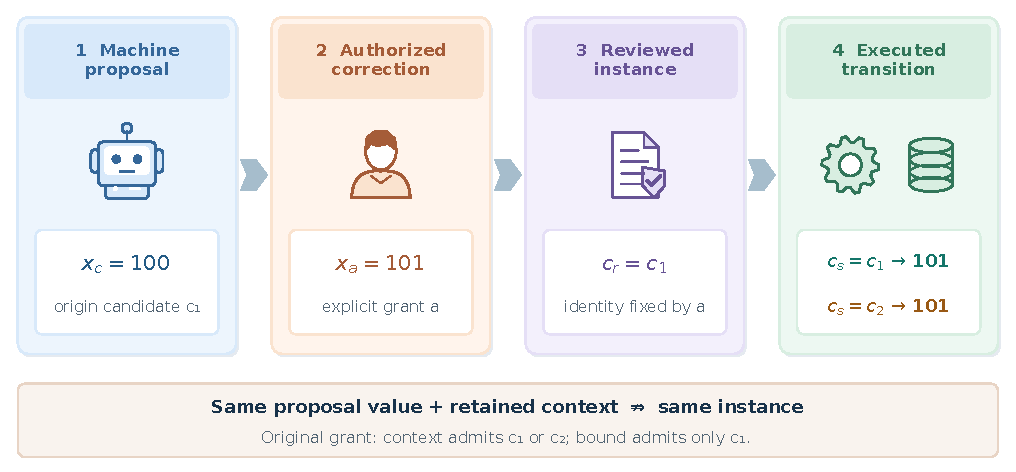
\includegraphics[width=\textwidth]{figures/revised-figure1-concept.pdf}
\caption{Correction-aware review-to-execution continuity. Review authorizes 101 from $c_1$ while retaining its proposal 100. Equivalent $c_2$ has the same value/context but a different identity. Context permits either instance under the original grant; bound permits only $c_1$. A new authorization can license $c_2$. This is a conceptual construction.}
\label{fig:contract}
\end{figure*}

\begin{figure*}[t]
\centering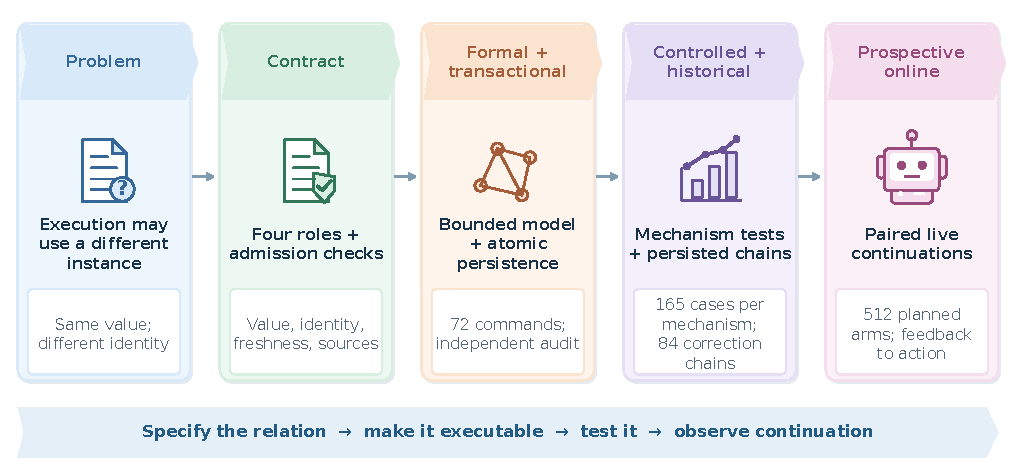
\includegraphics[width=\textwidth]{figures/revised-figure2-evidence-chain.pdf}
\caption{Evidence chain for trustworthy corrected execution. Distinct layers define continuity, make it executable, validate persistence and integration, then observe live agent continuation. Counts retain separate units: bounded commands, cases per mechanism, archived correction chains and planned paired trajectories.}
\label{fig:evidence}
\end{figure*}

\section{Introduction}
Agents that invoke tools increasingly change persistent operational state. They update records, publish revised values and commit results that later actions treat as authoritative. Trustworthy execution therefore requires an accountable connection between a state change and the review that authorized it. Human-in-the-loop frameworks already pause tool calls, permit argument edits and resume execution \citep{langchainHITL}. The open execution question is what must remain continuous while an agent acts after that review.

Correction makes this question concrete. A machine proposes $x_c$; a reviewer authorizes $x_a$. When a proposal of 100 is corrected to 101, the system should commit 101 and retain the original 100 as proposal evidence. Guided repair and interactive cleaning already distinguish system suggestions from human judgments \citep{yakout2011guided,he2016falcon}. In a state-changing agent workflow, the distinction extends across time: the system must retain both what was proposed and which reviewed instance is entitled to supply the later transition.

Suppose two persisted candidates, $c_1$ and $c_2$, propose 100 for the same field and retain the same evidence, producer and expected predecessor. They differ only in instance identity. A reviewer inspects $c_1$ and authorizes 101. The agent then obtains an equivalent preview, or receives a queued handoff carrying $c_2$, and executes it under the earlier grant. The value may still be 101. Every retained contextual check may agree. Under an instance-accountability requirement, however, the transition has crossed a review boundary: the candidate used for execution is not the one reviewed. Figure~\ref{fig:contract} separates value correctness from this review-to-execution relation.

Transactions, provenance and approval provide essential foundations. Transactions install atomic changes \citep{gray1981transaction}; concurrency control validates the predecessor \citep{kung1981occ}; provenance retains derivation and responsibility \citep{buneman2006curated,moreau2013provdm}; and authorization mechanisms bind approval to an executable request \citep{clark1987integrity,owaspTransactionAuthorization}. We bring these foundations together around corrected execution: the original proposal, the explicitly authorized replacement, the reviewed instance and the executed transition must remain distinguishable. Their relation also has a behavioral consequence. If enforcement rejects a continuation, the resulting feedback becomes input to an agent that must choose what to do next.

We ask: \emph{How should authorization preserve review-to-execution continuity when corrected agent proposals become persistent changes, and how does enforcement reshape subsequent execution and recovery?} Our answer combines an executable contract with a paired online intervention. The contract connects the four roles to freshness, complete successors and exact field sources. The intervention compares retained-context and instance-bound policies after the same reviewed history, following actual feedback through the next meaningful action, recovery path, task utility and integrity. Figure~\ref{fig:evidence} maps this argument from the motivating distinction to observed continuation.

The paper makes four contributions:
\begin{enumerate}[leftmargin=*,itemsep=2pt]
\item \textbf{Correction-aware continuity.} We define the four-role review-to-execution relation and construct histories that separate equal values and retained context from the identity of the reviewed instance.
\item \textbf{An executable authorization contract.} We integrate instance binding with predecessor freshness, atomic complete successors and field-level provenance, supported by bounded formal checks and independent persistence auditing.
\item \textbf{Cross-layer mechanism evidence.} Controlled comparisons establish policy separation and agreement across two exact-binding realizations; request-binding tests and archived hosted-agent corrections connect the contract to its integration boundaries.
\item \textbf{Online execution and recovery evidence.} A frozen paired intervention measures how authorization feedback changes subsequent agent actions, while reporting utility, integrity and operational friction separately.
\end{enumerate}

Three findings organize the paper. \textbf{Correction creates a distinct continuity problem}: a correct endpoint can preserve the wrong reviewed origin. \textbf{The relation is explicit and enforceable across persistence mechanisms}: formal constraints and transactional effects expose the same distinction. \textbf{Online enforcement redirects recovery with measurable friction}: all 17 exposed instance-bound handoffs recover with intact continuity, whereas context admits the substituted instances. Agent-managed refreshed previews show no observed substitution. Together, these findings connect a precise execution contract to the decisions an agent actually makes after feedback.

\section{Related Work}
\subsection{Agent approval and tool execution}
Approval mechanisms already control state-changing operations. Clark--Wilson combines authenticated execution, well-formed transactions and reconstructible audit records \citep{clark1987integrity}. Collaborative databases can retain cell versions pending approval, including approval tied to a cell identifier and timestamp \citep{mershad2015approval}. Current agent middleware interrupts selected tool calls and permits approval, edits or rejection before resumption \citep{langchainHITL}. Server-controlled authorization data and a final execution gate are established security guidance \citep{owaspTransactionAuthorization}. Our correction case concerns the relation among four roles after such a decision: the original proposal, the corrected authorized value, the reviewed candidate and the candidate used for execution. A completed approval step provides a starting point for that relation; the continuation determines whether it is preserved.

\subsection{Transactions, provenance and \mbox{governed} state}
Transactions and optimistic concurrency control support atomic successors and validation against current state \citep{gray1981transaction,kung1981occ}. Database provenance identifies contributing data and derivations \citep{buneman2001whywhere,cheney2009provenance}. Curated-database provenance records edits and copies across versions, including the connection of unchanged data to preceding versions \citep{buneman2006curated}; reenactment reconstructs transaction provenance \citep{arab2018reenactment}. PROV-DM models entities, activities, agents and their responsibility relations \citep{moreau2013provdm}. These mechanisms supply the persistence vocabulary for the execution contract. The authorization target still has to specify whether equivalent contents or a particular reviewed instance may supply a corrected transition. We implement the same contract with relational objects and an event journal so that this question is separated from storage representation.

\subsection{Trustworthy execution and \mbox{recovery}}
AgentDojo separates task utility from security outcomes in interactive tool environments \citep{debenedetti2024agentdojo}. Recent preprints also place authorization at the execution boundary. Cordon (Chen et al., 2026, \href{https://arxiv.org/abs/2606.17573}{arXiv:2606.17573}) stages local changes and external effects within a task-level transaction, with lineage, scoped approval and recovery. Continuity Kernel (He and Yu, 2026, \href{https://arxiv.org/abs/2608.11632}{arXiv:2608.11632}) binds proposal identity, predecessor state, pre-state authority and evidence to atomic state activation. Commit-time authorization (Santos-Grueiro, 2026, \href{https://arxiv.org/abs/2607.10487}{arXiv:2607.10487}) checks whether authority remains fresh, causally prior, effect-bound and eligible at durability, and separates authorized completion from endpoint success. Our comparison fixes the corrected value and retained context while varying whether execution must use the reviewed candidate instance. The contract preserves the machine value, authorized replacement and reviewed/executed identities as separate roles. Paired live continuations reveal how enforcing that relation changes the next action, recovery path and execution cost.

\section{Review-to-Execution \mbox{Continuity}}
\subsection{Four roles in a corrected state change}
Let $\Sigma_v$ be an authoritative record state with a nonempty field domain $F_r$, total values $V_v:F_r\to X$ and total durable sources $S_v:F_r\to T$. A persisted candidate is
\begin{equation}
c=\langle id,r,f,e,v_{\rm exp},x_c,p\rangle,
\end{equation}
where $id$ names the immutable instance, $r,f$ identify the target, $e$ identifies persisted evidence and its locator, $v_{\rm exp}$ is the expected predecessor, and $p$ identifies the producer. Retained context $K(c)$ includes the declared non-identity review information. Instance identity is not reconstructed from the proposal value or $K(c)$.

An authorization $a=\langle c_r,x_a,q\rangle$ records the reviewed instance $c_r$, explicit authorized value $x_a$ and authorized principal $q$, together with its validity information. A commit request submits $c_s$ and a value $x$. The roles obey
\begin{align}
\operatorname{proposal}(c_r)&=x_c,\nonumber\\
\operatorname{authorized}(a)&=x_a,\nonumber\\
\operatorname{committed}(\Sigma_{v+1},f)&\jeq x_a.
\end{align}
The committed transition retains the proposal as origin evidence and the authorization as the authority for the chosen value. Correction permits $x_c\jneq x_a$; it does not rewrite the immutable proposal to make the two values appear equal.

Contract value comparisons use canonical JSON equality, written $\jeq$: sorted-key, whitespace-minimal serialization must agree. Consequently, an integer, a floating-point serialization and a Boolean remain distinguishable when their serialized values differ. This equality is shared by change detection, admission value checks, tracing and the independent oracle.

\subsection{Content agreement and reviewed-instance continuity}
For an already issued authorization, define
\begin{align}
K_{eq}&\iff K(c_s)=K(c_r),\nonumber\\
I_{eq}&\iff id(c_s)=id(c_r).
\end{align}
Let $G$ collect the remaining disclosed checks: authorization validity, predecessor freshness, committed-value equality, evidence integrity, successor shape, source relations, transaction constraints and grant consumption. It excludes an implicit instance comparison. The two execution policies are
\begin{align}
P_\context&: \operatorname{Admit}=G\land K_{eq},\label{eq:context}\\
P_\bound&: \operatorname{Admit}=G\land K_{eq}\land I_{eq}.\label{eq:bound}
\end{align}
Both retain the reviewed identifier. Only the decision to require its equality at execution differs. Context-equivalent $c_2$ can therefore pass Eq.~\ref{eq:context} under $c_1$'s authorization while failing Eq.~\ref{eq:bound}. This is a policy separator under a declared instance-accountability requirement. Context-based authorization remains a coherent choice for an application whose responsibility contract treats those instances as interchangeable.

\subsection{Failure-distinguishing information}
To identify which distinctions the contract must retain, the declared failure model separates five information classes: candidate identity/context ($D_C$), proposal/authorized-value attribution ($D_V$), predecessor freshness ($D_F$), complete atomic successor ($D_B$), and total field sources ($D_S$). For a history $h$, $\pi_I(h)$ retains the specified logical observations in $I$, and $O(h)$ assigns the full-history authority outcome, including successor and trace status. Candidate handles are opaque: a reduced observation cannot recover an omitted class by decoding an identifier.

\paragraph{Proposition 1: class-wise irredundancy.}
For every $d\in\mathcal D=\{D_C,D_V,D_F,D_B,D_S\}$, the declared model contains paired histories satisfying
\begin{equation}
\pi_{\mathcal D\setminus\{d\}}(h_s)=\pi_{\mathcal D\setminus\{d\}}(h_u),
\quad O(h_s)\ne O(h_u).
\end{equation}
Thus a decision based on the reduced observations cannot distinguish both required outcomes.

\paragraph{Construction.}
Hold the other observations fixed while changing, respectively, candidate/context binding, the authority assigned to a corrected value, the entry-time predecessor comparison, the single-versus-fragmented commit sequence, or one required source anchor. Each pair changes the corresponding derived authority outcome. A fixed-registry pair further selects either the reviewed candidate or a context-equivalent alternative while retaining the same two candidates and non-identity information. It isolates instance continuity within $D_C$. Observation functions and valid histories are specified independently; the checker derives projections and outcomes from complete relations. This establishes class-wise irredundancy within the declared failure model. Full constructions and projection assumptions are in the supplement.

\subsection{Atomic successors and exact source preservation}
For an admitted nonempty batch $B$ with unique changed fields, the required effects are
\begin{equation}
\Delta(V_v,V_{v+1})=\{i.f:i\in B\}=\{t.f:t\in T_{v+1}\}.
\end{equation}
Each admitted item has one transition to its explicitly authorized value; all items share the target record, observed predecessor and one successor. Initial coverage establishes complete value/source domains. Later admissions preserve every unchanged field's value and exact source:
\begin{equation}
f\notin\Delta\Rightarrow V_{v+1}(f)\jeq V_v(f),\quad S_{v+1}(f)=S_v(f).
\end{equation}
Decision, authorization binding, transitions, complete version, sources and audit effects commit together, or the authoritative state stutters. Candidate and review preparation already persisted before the attempted admission remain historical evidence. Online Resource 1, Section S2 states the full P0--P6 contract, no-op handling and mixed-submission semantics.

\section{Formal and Transactional \mbox{Realization}}
\subsection{Making the relation executable}
The relational model encodes candidates, evidence, principals, authorizations, ordered versions, complete states and source transitions. Machine events may extend candidates and evidence while framing authoritative state. Full admission adds binding, freshness, complete shape and item--transition correspondence to the base state change. Removing a conjunct while retaining another valid item exposes which required distinction that conjunct enforces. Alloy and Kodkod make these finite relational checks executable \citep{jackson2002alloy,torlak2007kodkod}. The independent concrete-to-relational mapping follows the abstraction/concretization testing principle exemplified by TestEra \citep{marinov2001testera}.

The archived checks cover legal admissions, conjunct-removal witnesses, source attacks and nonempty trace-preservation premises. All 72 command outcomes agree with their manifests across two scope profiles. The assertion checks have no counterexamples within their encoded finite scopes. An independent abstraction reads persisted pre/post relations, maps them into fixed instances, and checks Full admission or rejected-state stutter: nine intended projections are satisfiable and twenty selected mapping mutants are unsatisfiable. The supplement records exact scopes, commands, assumptions and concrete/formal domain differences.

\subsection{Transactional persistence and review binding}
\system{} separates candidate-writing capability from authoritative admission. An immutable certificate includes the persisted candidate instance and its canonical target, proposal, producer, expected predecessor and evidence identity. A review decision binds that certificate to the explicit authorized value. Field transitions retain the chain through both accepted and corrected proposals.

The relational adapter reloads the current field domain, complete predecessor, evidence and authorization within the transaction. It derives changed fields using canonical equality, validates exact bindings and unused identities, checks the principal policy, and compares-and-swaps the expected version. It then writes one transition per admitted field and copies exact unchanged sources into one complete successor. Constraints reinforce unique transitions and coherent references. Any unsuccessful attempt stutters relative to the immediately preceding authoritative database state.

A separately implemented event journal stores the same authority-relevant relations. Its retained-context configuration omits instance equality at the execution gate; its exact configuration adds the reviewed-candidate link. Comparing the exact journal with the relational implementation tests the same contract across storage representations. Comparing the two journal configurations isolates the binding choice within one representation.

Faithful transfer of review requires a binding before the final request arrives. A server-held review record can fix the candidate, expected version, reviewer and corrected value, then validate the request against that record. The resulting guarantee concerns request-to-record consistency. Browser presentation is a separately observable layer: a page can display a different candidate while the server and request still name the recorded one. Controlled request and display probes identify that boundary.

\subsection{Independent audit of authoritative effects}
The source verifier follows every field through its exact transition, authorization, candidate certificate, producer, evidence and predecessor. Changed fields need their unique new transition; unchanged fields retain the preceding source. A separate database oracle reads persisted relations rather than trusting the production planner or trace builder. Rejection checks compare full logical database digests, and corruption probes require changed state plus a diagnosis. These checks connect the written contract to the actual durable successor.

The prospective experiment uses another independent oracle for the paired policies. It checks raw responses against executed tool actions, hash-linked events, persisted state snapshots and reviewed-history provenance. Integrity is determined from authoritative transitions and audit coverage, rather than from a gate's own claim that an operation was admissible. This permits a context-admitted transition to satisfy its policy while violating the separately declared instance-continuity oracle.

\section{Controlled and Historical Evidence}
\subsection{Controlled mechanism and system validation}
Context-equivalent substitutions separate reviewed-instance continuity from content approval. The archived E1 comparison executes 165 cases per mechanism. The context journal accepts all fifteen same-value/same-context substitutions; the exact journal and relational reference reject them. The two exact mechanisms agree on all corresponding decisions and provenance-query answer sets. Each accepts 45 legal cases and rejects 120 with authoritative-state stutter. This establishes the executable separator that the online experiment subsequently turns into agent-visible feedback.

\begin{table}[t]
\centering\small
\caption{Controlled mechanism evidence. Counts retain their original interpretation units; all cases are constructed or scripted.}
\label{tab:controlled}
\begin{tabularx}{\columnwidth}{@{}lX@{}}
\toprule
Evidence & Observed result \\
\midrule
Persistence binding & Exact journal/reference agree in 165 cases; context accepts 15 instance substitutions \\
Request binding & Server-held gate rejects 9 request substitutions accepted by original path \\
Display boundary & Both paths accept 3 display-only substitutions \\
Formal/concrete checks & 72 bounded commands match; 9 intended projections SAT; 20 mapping mutants UNSAT \\
\bottomrule
\end{tabularx}
\end{table}

Server-held review binding separates request substitution from faithful presentation. E2 has thirty browser cases per path: nine legitimate controls, nine request substitutions, nine stale/replay/interrupted controls and three display-only substitutions. The gate rejects every request substitution while preserving the legitimate controls. Both paths reject the stale, replay and interrupted cases without fact writes. Both admit the display-only controls because their actual request still matches the server record. Table~\ref{tab:controlled} groups this evidence under one realization question.

The persistence contract also makes implementation cost measurable. Complete confirmation and source reconstruction are timed separately, with exact output agreement checked across the 36 paired trace-workload cells. Online Resource 1, Section S4 retains the complete admission, tracing and storage grids and their timer boundaries. Agent-level friction is measured after the online policy intervention, where the additional work is an observed part of continuation.

\subsection{Observable correction in hosted workflows}
The correction contract is recoverable from archived hosted-agent persistence. A new audit of 1,260 historical databases identifies 84 retained machine-origin correction chains, checking 252 evidence associations, 168 record versions and 168 reconstructed provenance traces. Each chain preserves a machine proposal, explicit host-authorized correction, exact candidate binding and persisted transition. These chains provide integration evidence for the role distinction defined in Section 3.

The audit unit is a persisted correction chain rather than whole-task success. The corresponding archived endpoints include 80 strict-safe task successes, one safe utility failure, two model/API failures and one timeout. All 84 persisted chains satisfy the audited relation. Their single-field cases provide zero unchanged-field checks, so copy-forward is supported by the controlled multi-field evidence. Full original task and annotation denominators remain in the supplement, separate from the prospective policy experiment.

\section{Prospective Online Agent Experiment}
Controlled mechanism separation establishes that the policies differ, but it does not tell us what happens once that difference becomes feedback to an adaptive agent. The prospective experiment compares Eqs.~\ref{eq:context} and \ref{eq:bound} in live continuations. It is designed around the sequence
\begin{equation}
\begin{aligned}
\text{feedback}&\to\text{next agent action}\\
&\to\text{recovery path}\to(U,I).
\end{aligned}
\end{equation}
The local precollection freeze fixes the tasks, pair order, deployments, prompts, tools, resource rules, scorer and failure handling. The separately archived pilot supports engineering readiness and is excluded from formal effect analysis.

\subsection{Shared review history and unique policy difference}
A shared prospective prefix isolates the post-review continuation effect by giving both policies the same reviewed history (Figure~\ref{fig:loop}). An actual agent proposes and obtains host review; the complete visible conversation and persisted state are then copied into isolated policy arms. The same task, checkpoint, tools, deterministic reviewer, persistence, prompt and resource-policy family apply to both arms. This isolates the effect of requiring $I_{eq}$ on subsequent continuation. Both arms retain the reviewed identifier, so the comparison changes its use at execution rather than its availability for auditing.

A deterministic host reviewer fixes the correction decision across arms, separating authorization consequences from variation in review judgments. Two independently accessed deployments expose the same contract through distinct provider routes, with complete request-level provenance. Configuration A uses the frozen account-backed Codex route; B uses the recorded compatible API route. Requested aliases, observed returned identifiers, settings and collection timestamps are retained in the supplement and artifact. The common action interface presents the same tool definitions and returns actual results to subsequent decisions.

Each task/configuration forms one adjacent context/bound pair. A frozen assignment manifest balances which policy runs first within scenario and configuration. Two provider lanes execute one pair each, respecting this order. All planned arms remain in the analysis ledger, with runtime outcomes and audit coverage recorded separately. The supplement specifies the collection and interruption rules.

\begin{figure*}[t]
\centering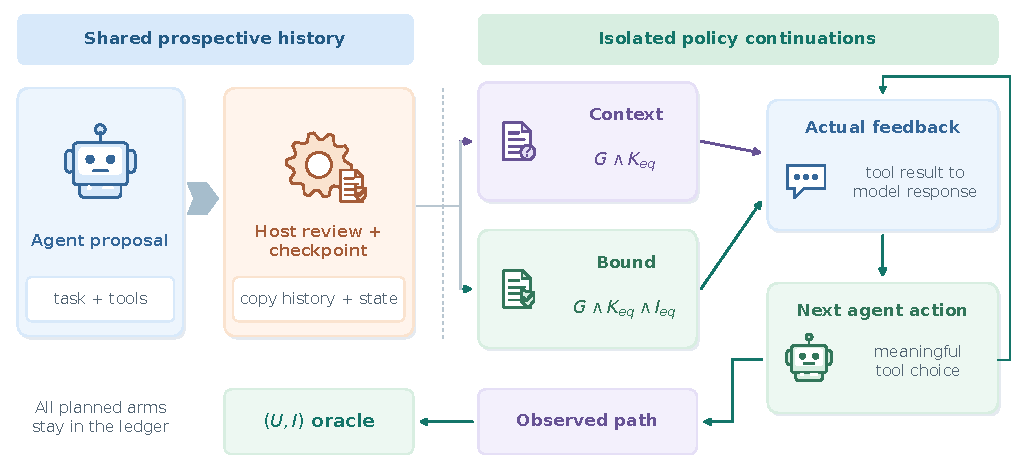
\includegraphics[width=\textwidth]{figures/revised-figure3-online-loop.pdf}
\caption{Paired online intervention after a shared prospective review. The visible conversation and persisted checkpoint are copied into isolated policy arms. The only execution-rule difference is $I_{eq}$. Actual tool feedback enters the next sampled agent decision, whose actions and terminal state are independently audited. The standardized G handoff supplies an index request; N instead leaves refreshed-preview management to the agent.}
\label{fig:loop}
\end{figure*}

\subsection{Task families and controlled exposure}
The design contains 128 task instances, two configurations and two policies: 256 paired units and 512 planned policy trajectories, with one repetition. Controlled correction tasks expose specific authorization boundaries while keeping legal recovery paths interpretable. Their frozen distribution is
\[
L32+N32+G16+E16+V16+R16=128.
\]
\begin{description}[leftmargin=0pt,itemsep=2pt]
\item[L: legal correction.] Execute the reviewed instance with the corrected authorized value; check ordinary completion and nonvacuous unchanged-source preservation.
\item[N: refreshed preview.] After authorization, the agent obtains a required refreshed preview and decides how to preserve continuity. It can reuse the reviewed instance, authorize a new candidate or otherwise manage the workflow; the harness does not force an invalid commit.
\item[G: queued handoff.] The harness creates a same-value/same-context new instance and performs one standardized index action under the prior grant. Its actual result becomes feedback for autonomous continuation. The index action is marked \texttt{harness\_handoff}; it is a standardized recovery probe.
\item[E: changed evidence.] Publish changed evidence bytes and locator while preserving the proposal value. Both policies enforce the shared evidence/context checks; recovery can obtain a candidate reviewed against current evidence.
\item[V: stale predecessor.] Advance authoritative state externally. A fresh-state read, proposal and authorization provide a legal recovery path while preserving the externally updated source.
\item[R: unavailable receipt.] After a successful commit, the first receipt path is unavailable while authoritative state remains readable. Distinguish state confirmation, exact idempotent retry and semantic replay of a consumed grant.
\end{description}
The task generator varies business template, correction direction/magnitude, value relations, evidence layouts/locators, sources, version/history depths, retained metadata, candidate envelopes, snapshot organization, ordering and task wording. All 128 parameter vectors and rendered inputs are frozen. These variations diversify instances while preserving the six mechanisms.

\subsection{Utility, integrity and recovery}
Task utility $U=1$ requires the authoritative goal, required workflow actions and an accurate final report. Integrity is independently scored as $I\in\{1,0,\mathrm{unknown}\}$. Covered authoritative transitions must satisfy authorization, freshness, evidence/context integrity, authorized-value equality, provenance, copy-forward and the declared instance-continuity requirement. A proved violation yields $I=0$; incomplete necessary evidence yields unknown unless a violation is already proved. Runtime failure or rejected execution does not alone determine integrity.

Joint outcomes retain $(U,I)=(1,1),(1,0),(0,1),(0,0)$ and integrity unknown. A policy-admissible context substitution can therefore complete the task while failing the instance oracle. Completion and integrity are never collapsed into a total score.

A rejection is recoverable when its feedback is delivered and a legal path exists at the recorded rejection-time state. Delivery requires an actual received next model response with the recorded feedback input. Recoverability is determined from that state and available capabilities, not inferred backward from eventual success. The event-order classifier records the next meaningful tool action and observed reuse, verification, reproposal, reauthorization, state/evidence refresh, repeated invalid attempts, abandonment, confirmation and terminal failure. Raw component actions remain available alongside the primary path label. Every $U=0$, $I=0$ or unknown arm enters the complete failure-archaeology ledger.

\subsection{Paired effects and operational components}
Two primary endpoints are frozen: $\Delta U=U_\bound-U_\context$ and the bound-minus-context difference in run-level instance-continuity failure incidence. Transition-level executed substitution is a separate diagnostic. Unknown continuity contributes explicit identification bounds rather than a zero replacement.

For aggregate effects, each task contributes its average configuration-specific paired difference. A scenario-stratified bootstrap resamples 128 task clusters, retaining both configurations and both policies; the frozen plan uses 10,000 iterations and seed 20261007. Separate configuration-specific exact McNemar tests are secondary. The structure supplies paired effects and controlled-task uncertainty, rather than 512 independent samples.

Recovery distributions conditional on delivered rejection are descriptive because exposure is post-treatment. G-bound provides the standardized probe cohort; N remains a separate account of agent-managed continuity. Operational components report additional tool calls, model turns, authorization attempts, reproposals, verifications, elapsed time and observed provider usage. Unsuccessful runs retain the specified budget-capped time-to-success alongside their actual termination time. Shared-prefix provider usage is charged once per pair. No arbitrary composite friction score is introduced.

\section{Results}
\subsection{Continuity and task completion}
Instance-bound execution separates accountable completion from successful state mutation in the standardized handoff tasks. The complete ledger contains 256 terminal pairs and all 512 planned arms. Context has 17 proved instance-continuity violations, all in G: sixteen in B and one in A. Bound has no proved violations; one bound arm and one context arm have unknown integrity. Fifteen context violations accompany successful task completion, and two accompany unsuccessful completion. The distinction between $U$ and $I$ therefore changes the interpretation of an apparently successful run.

\begin{table*}[t]
\centering\small
\caption{Complete planned-ledger outcomes. Every row contains 128 arms. A covered run without an unauthorized transition can have $I=1$ despite unsuccessful execution. Unknowns are the two N arms affected by the initial infrastructure interruption.}
\label{tab:joint}
\setlength{\tabcolsep}{4pt}
\begin{tabular}{@{}llrrrrrrr@{}}
\toprule
Deployment & Policy & $U=1,I=1$ & $U=1,I=0$ & $U=0,I=1$ & $U=0,I=0$ & $I$ unknown & $U=1$ & Checkpoint pairs \\
\midrule
A & Context & 8 & 1 & 119 & 0 & 0 & 9 & 11/128 \\
A & Bound & 9 & 0 & 119 & 0 & 0 & 9 & 11/128 \\
B & Context & 103 & 14 & 8 & 2 & 1 & 117 & 128/128 \\
B & Bound & 119 & 0 & 8 & 0 & 1 & 119 & 128/128 \\
\bottomrule
\end{tabular}
\end{table*}


The reviewed checkpoint is reached in 11 of A's 128 pairs and all 128 of B's pairs. In A, 117 prefixes terminate after provider quota exhaustion. Both arms inherit that shared-prefix failure, yielding 234 unsuccessful planned arms with covered state and no unauthorized transition. Four further A suffixes terminate with runtime errors. B has eighteen malformed-output terminations across the two policies. The initial file-replacement interruption leaves one partial context arm and one unstarted bound arm with unknown integrity. These outcomes remain in Table~\ref{tab:joint}, rather than being replaced with newly sampled tasks.

The paired completion estimate is small relative to its task-cluster uncertainty. Context completes 126/256 arms (49.22\%) and bound 128/256 (50.00\%). The frozen task-averaged bound-minus-context effect is $+0.78$ percentage points, with 95\% interval $[-1.95,3.52]$. In B, the corresponding counts are 117/128 and 119/128, an effect of $+1.56$ points with interval $[-3.91,7.03]$. Five B tasks complete only under context and seven only under bound; the secondary exact McNemar test gives $p=0.774$. A has nine completions per policy. The intervals quantify variation over the paired controlled tasks and retain both deployments' resource outcomes.

The planned-ledger continuity comparison favors bound throughout the identification interval allowed by the unknown outcomes. Across the complete planned ledger, the bound-minus-context difference in continuity-failure incidence lies in $[-7.03,-6.25]$ percentage points. Online Resource 1, Section S11 reports bootstrap uncertainty for each endpoint, keeping the two unknown arms explicit. At the transition level, all seventeen observed substitutions are policy-admissible under context and instance-incompatible under the independent oracle. The remaining shared guard and provenance checks hold for these transitions. The improvement thus concerns the disclosed extra continuity obligation, rather than correcting a context policy's own decision rule.

\subsection{Feedback, next actions and recovery paths}
Delivered instance-mismatch feedback redirects every exposed G-bound continuation toward an authorized execution path. The standardized handoff reaches seventeen of the 32 planned G pairs: sixteen in B and one in A. Each context index action accepts the new instance under the old reviewed grant. Each paired bound index action rejects it, and each rejection is proved delivered to an actual subsequent provider response. Legal recovery exists at all seventeen rejection states. All seventeen bound continuations end with $(U,I)=(1,1)$, whereas the context continuations retain the irreversible instance violation even if later actions report the correct goal.

Reviewed-candidate reuse accounts for all sixteen B recoveries. Their first meaningful action after rejection is \texttt{commit} using the original reviewed candidate and grant. They neither regenerate evidence nor request a new authorization to solve this mismatch. A's one delivered continuation instead requests authorization for the handoff candidate and then commits it. These are two distinct legal responses to the same continuity obligation. The counts describe actual observed responses: the host exposes the mismatch but does not prescribe either repair sequence.

\begin{figure*}[t]
\centering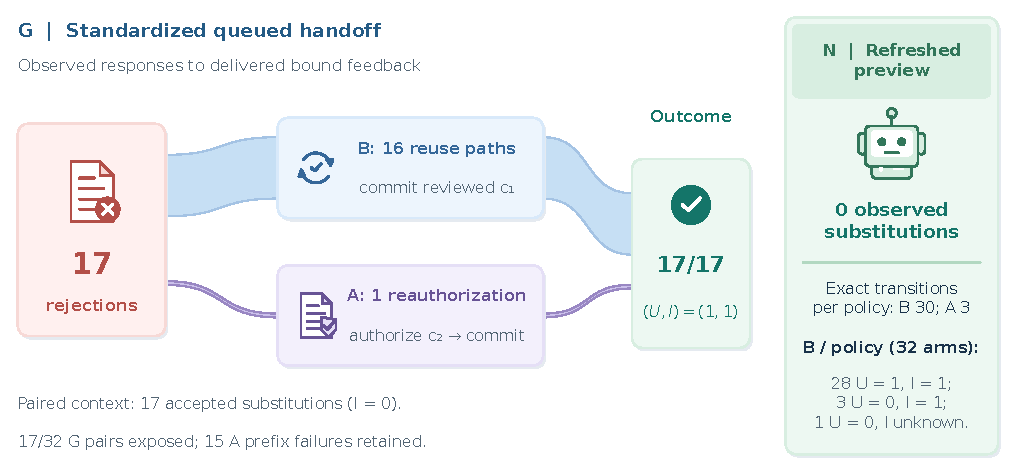
\includegraphics[width=\textwidth]{figures/revised-figure4-recovery-paths.pdf}
\caption{Observed paths after standardized mismatch feedback. All 17 exposed G-bound continuations recover with $(U,I)=(1,1)$: B reuses the reviewed candidate in 16 cases, and A reauthorizes the handoff candidate in one. The separate N panel retains agent-managed preview outcomes and unknown coverage. The figure reports observed paths, not the frequency of naturally occurring substitutions.}
\label{fig:paths}
\end{figure*}

Agent-managed refreshed previews preserve reviewed-instance continuity under both policies in every covered N transition. B has thirty such transitions per policy, all using an instance compatible with the review; A has three per policy. B completes 28 of its 32 N arms under each policy. Each B policy also has three covered unsuccessful arms and one unknown arm. No delivered instance-mismatch feedback occurs in N. Figure~\ref{fig:paths} keeps this absence of voluntary mismatch separate from G's deliberately exposed handoff. The observed behavioral consequence of the unique policy conjunct is concentrated in G, rather than appearing throughout ordinary preview continuation.

Evidence, version and receipt boundaries induce different observed recovery actions through the shared execution contract. In B, E supplies sixteen delivered evidence rejections per policy; fifteen continuations per policy obtain a fresh proposal and authorization and complete. V supplies thirteen delivered stale-version rejections per policy; twelve per policy recover through a current-predecessor proposal and review. The first V action varies between reading state and immediately proposing from available updated information. In R, nine context and ten bound receipt failures are proved delivered; nine continuations in each policy confirm success through state. One further bound run makes no subsequent tool action and still provides an accurate completed report, so the frozen episode classifier records no observed recovery endpoint for that episode. Run-level completion and the stricter episode recovery label remain separate.

\begin{table*}[t]
\centering\small
\caption{Delivered-feedback continuations in B. Each row's denominator is delivered episodes, not all planned tasks. All listed episodes have a legal path at rejection time. E, V and R involve shared checks/capabilities; only G exposes the policies' unique instance rule. Recovery requires a recorded recovery endpoint, $U=1$ and $I=1$.}
\label{tab:recovery}
\begin{tabularx}{\textwidth}{@{}llrrXX@{}}
\toprule
Family & Policy & Delivered & Recovered & First meaningful action & Observed path \\
\midrule
G & Bound & 16 & 16 & Commit (16) & Reuse reviewed candidate (16) \\
E & Context & 16 & 15 & Inspect evidence (15), propose (1) & Fresh proposal and authorization (15) \\
E & Bound & 16 & 15 & Inspect evidence (16) & Fresh proposal and authorization (15) \\
V & Context & 13 & 12 & Propose (7), state read (5), none (1) & Fresh proposal and authorization (12) \\
V & Bound & 13 & 12 & State read (10), propose (2), none (1) & Fresh proposal and authorization (12) \\
R & Context & 9 & 9 & State read (9) & State confirmation (9) \\
R & Bound & 10 & 9 & State read (9), none (1) & State confirmation (9) \\
\bottomrule
\end{tabularx}
\end{table*}

The event-order analysis separates successful repair strategies from unsuccessful continuation and absent behaviors. It identifies reuse, reproposal, reauthorization, state refresh and evidence refresh. No delivered episode is labeled reverify, repeated-invalid, fresh-id-invalid-loop, stale-reuse, hallucinated-success or timeout. Terminal malformed output and runtime interruption account for unsuccessful observed continuations; no frozen \texttt{abandon} label occurs. Table~\ref{tab:recovery} describes paths conditional on delivered feedback; the primary contrast remains the paired policy comparison on the planned ledger.

\subsection{Operational friction and complete failure archaeology}
The standardized continuity repair adds an explicit execution action even when task completion is preserved. Across B's sixteen G pairs, bound uses exactly one additional agent tool call per pair, with no additional authorization requests. The median paired suffix-time difference is $+14.54$ seconds; its mean is $+8.84$ seconds. Model turns increase by a mean of 0.94. The one exposed A pair instead adds two tool calls, including one authorization request. The difference between reuse and reauthorization is therefore visible as an execution cost rather than merely as an extra rejection count.

\begin{table}[t]
\centering\small
\caption{B's paired operational components (bound minus context). ``All'' uses 127 pairs with both suffix records; G uses all 16 pairs. Elapsed time includes unsuccessful suffixes. Median and mean time answer different questions.}
\label{tab:friction}
\begin{tabular}{@{}lrr@{}}
\toprule
Component & All & G \\
\midrule
Mean extra agent calls & 0.071 & 1.000 \\
Mean extra model turns & 0.039 & 0.938 \\
Mean extra authorizations & 0.000 & 0.000 \\
Median extra suffix seconds & 0.69 & 14.54 \\
Mean extra suffix seconds & 1.29 & 8.84 \\
\bottomrule
\end{tabular}
\end{table}

Operational differences concentrate at the exposed boundary rather than uniformly increasing every component. Across B's 127 complete suffix pairs, mean extra agent calls are 0.071, mean extra model turns 0.039 and mean extra authorizations zero; median extra elapsed time is 0.69 seconds. The 720-second budget-capped time-to-success endpoint retains all 128 B pairs and has mean paired difference $-9.74$ seconds. In G its mean is $-76.53$ seconds, despite positive median elapsed friction, because two unsuccessful context reports receive the unsuccessful-run cap while all bound runs complete. A favorable capped endpoint therefore does not imply faster execution. The supplementary component table retains actual time, capped time and provider usage separately, with the shared prefix charged once.

The all-arm archaeology contains 273 distinct arms with $U=0$, $I=0$ or unknown integrity. They partition into 238 A runtime failures, fifteen successful context arms with an instance violation, two unsuccessful context arms with an instance violation, sixteen further unsuccessful B arms with covered intact integrity, and two unknown N arms. The unsuccessful B arms comprise eighteen malformed-output terminations overall, two of which also have the G continuity violation. Infrastructure interruption accounts for the remaining two unknown arms. Every violating transition is in G; no proved evidence, value, freshness, source-preservation or copy-forward violation accompanies it. The full ledger includes identities, stage, terminal type, component labels, missing coverage and the underlying episode records before any trajectory is selected for illustration.

The online results describe controlled correction workflows, with most live continuation evidence supplied by B and eleven reviewed checkpoints in A. G measures recovery after a standardized mismatch, while N records voluntary continuity management; neither estimates natural substitution prevalence. A separately frozen quota-recovery cohort is incomplete in the available snapshot (45 of 117 selected A pairs terminal) and is excluded from all results above. Online Resource 1, Section S12 preserves its separate status and integration requirements.

\section{Discussion and Limitations}
\subsection{What continuity adds to corrected execution}
Correction makes the authority for a value distinct from the origin of its proposal. Preserving only the final corrected value loses the machine output; preserving only the proposal loses the reviewer-authorized replacement. Retaining both still leaves the identity question: which candidate did the authorization cover, and which supplied the actual transition? The context-equivalent separator shows why those roles cannot be reconstructed from a successful endpoint alone. The fifteen $(U,I)=(1,0)$ trajectories provide an online counterpart to that distinction: meeting the task goal and retaining the authorized value does not establish review-to-execution continuity.

This account gives established system mechanisms a common execution target. Transactions make the complete successor atomic. Provenance makes its effects reconstructible. Version validation controls the predecessor against which it is installed. Instance authorization determines which reviewed origin may supply that successor. Their joint contract supports the correction case without equating machine proposal and authorized value. The controlled agreement across relational and event-journal realizations shows that the relation can survive a change of representation; the hosted-chain audit shows that its roles can be recovered from persisted integration evidence.

\subsection{Authorization as part of the execution environment}
An authorization rule has behavioral consequences when its result becomes input to the next agent decision. In G, the difference between the policies is first mechanical: the same standardized request is accepted or rejected. The subsequent difference is an observed continuation. B responds by selecting the already reviewed candidate; A's available continuation obtains a new review. The gate does not generate those actions for the agent. It makes a continuity boundary visible, after which the agent selects an available legal path.

The contrast with N clarifies the mechanism's place in an agent system. A refreshed preview creates the possibility of identity substitution but does not force the agent to exploit it. Covered N transitions preserve the reviewed instance even when the looser policy would accept a context-equivalent alternative. The contract therefore performs two functions: it documents accountability when the agent already maintains continuity and supplies actionable feedback when a queued handoff breaks it. An execution-layer benefit can be material even when voluntary mismatch is absent in the agent-managed cohort.

The broader recovery results also separate obligations from repair sequences. Changed evidence calls for a current evidence-based proposal and review; a stale predecessor calls for a current-state proposal; an unavailable receipt can be resolved by confirming state rather than applying another mutation. These paths use the same tool vocabulary but solve different contract boundaries. A useful execution environment should expose which relation failed and retain the state needed for a legal next step. Rejection frequency alone omits whether the agent received that information, acted on it and reached an accountable outcome.

\subsection{Accountability and execution cost}
The measured trade-off is additional execution work at a standardized continuity boundary, alongside improved instance accountability. The strongest direct result is B's G cohort: one extra agent call restores the reviewed link in every exposed pair, with a positive median suffix-time cost. Reauthorization is another legal strategy, but its one observed instance has a different call structure. These components matter operationally because a system can choose which recovery capabilities to expose and which authorizations remain reusable.

The overall completion interval leaves both modest improvement and modest loss compatible with the data. The continuity benefit therefore comes with an unresolved completion trade-off and a measured repair cost. The capped time endpoint rewards accurately completed reports, while actual suffix time captures latency. Reporting separate calls, turns, review requests, elapsed time and $U/I$ keeps these meanings visible. Provider failures additionally show why run completion, mutation integrity and availability need separate measurements: a covered run can leave state intact while accomplishing nothing.

\subsection{Scope and further evaluation}
The task family provides controlled exposure to six correction and execution boundaries, with one repetition of each task/configuration/policy combination. The deterministic reviewer fixes correction and authorization decisions, isolating execution binding from variation in human judgment; evaluations with interactive reviewers could additionally measure review burden and disagreement. The 128 tasks diversify inputs within those mechanisms, while broader business workflows, longer horizons and additional tools would test how the same contract interacts with a richer execution environment. The experiment measures controlled effects rather than production prevalence.

Deployment-level conclusions follow actual coverage. A reaches eleven checkpoints and contributes only one standardized mismatch recovery; B supplies the principal online evidence. Provider aliases and recorded settings support reconstruction of the accessed routes, while unavailable immutable model revisions constrain exact response reproduction. The frozen inputs, received responses, checkpoints and independent scorer support retrospective verification of the reported transitions and paths. The separate quota-recovery cohort can extend A's observed checkpoint coverage once complete; its selected failures and later collection conditions require separate reporting. Additional prospectively frozen deployments would test the stability of strategy choices and completion costs across provider revisions and resource conditions.

\section{Conclusion}
Correction-aware review-to-execution continuity separates what an agent proposed, what a reviewer authorized, which candidate was reviewed and which supplied a persistent transition. Formal relations, transactional realization and independent auditing make that distinction executable across persistence representations. Controlled and historical evidence establish the mechanism and its observable integration roles.

The complete prospective ledger connects the contract to live continuation. Standardized handoffs expose seventeen instance violations under context authorization; bound execution rejects those handoffs and all seventeen exposed continuations complete with intact continuity through reviewed-candidate reuse or fresh authorization. Agent-managed preview tasks produce no observed substitutions. Recovery adds measurable execution work, and the paired completion uncertainty leaves the utility trade-off open. Enforced inside an agent loop, review-to-execution continuity becomes actionable feedback that can redirect execution and expose the cost of accountability. This work makes that continuity explicit, enforceable and empirically observable in state-changing agent workflows.

\section*{Statements and Declarations}
\subsection*{Data and software availability}
The study uses constructed tasks and public lifecycle inputs. The controlled experiment archive is fixed at commit \href{https://github.com/lhh666-6/auto-dete/tree/2645e5e18c900ea91c9c980e44195dc71e410432/DKE-supplement}{\nolinkurl{2645e5e18c900ea91c9c980e44195dc71e410432}}. The reference implementation, formal models and earlier historical evidence are retained at commit \href{https://github.com/lhh666-6/auto-dete/tree/c6d512843c905cab6d8521dd8c914f7fb26d85ae/latest}{\nolinkurl{c6d512843c905cab6d8521dd8c914f7fb26d85ae}}. The prospective inputs and runner are fixed at master hash \nolinkurl{7773563b40c8db30d6def121915f50fbad032537edde32afd4ba39ec3eea744b}. The handoff archive at commit \href{https://github.com/lhh666-6/auto-dete/tree/475e66f549613aaaaa62c2ec81ffdee483636c54/cloud-handoff}{\nolinkurl{475e66f549613aaaaa62c2ec81ffdee483636c54}} retains the complete original formal ledger, raw responses, state snapshots, scorer, tables, figure sources and file hashes; Online Resource 1 maps the layers and reproduction steps. Reanalysis requires no new model calls. New hosted runs require provider access.

\subsection*{Ethics approval and consent to participate}
The prospective experiment uses constructed tasks and a deterministic host reviewer, with no new human participants. In the historical annotation study, one author (X.W.) and one non-author volunteer independently coded benign completion outcomes; L.H. adjudicated their disagreement and separately reviewed eleven human--rule disagreements. X.W. also completed the textual-acknowledgment annotation. Only pseudonymous annotator identifiers were collected. Both coders were informed of the task and data use, and the non-author coder participated voluntarily. The authors assessed the annotation of generated outputs as not requiring ethics approval. No animal subjects were involved.

\subsection*{CRediT authorship contribution statement}
Liang Hanghao: Conceptualization, Methodology, Software, Formal analysis, Investigation, Data curation, Validation, Visualization, Project administration, Writing--original draft, and Writing--review \& editing. Xuan Wentao: Methodology, Formal analysis, Investigation, Data curation, Validation, Visualization, and Writing--review \& editing. Chen Qile: Investigation and Validation. Peng Peng: Supervision and Writing--review \& editing.

\subsection*{Funding and competing interests}
This research received no external funding. The authors declare no competing interests.

\subsection*{AI-assisted preparation}
DeepSeek, OpenAI Codex and Claude assisted with code, analysis checks, literature organization and manuscript preparation. OpenAI tools assisted with manuscript reconstruction, offline evidence checks and figure scripts. An earlier diagram prototype used OpenAI image generation with an unrecorded model version; the present figures are rendered from explicit plotting scripts. AI tools are not authors. The authors retain responsibility for the article and its evidence.

\subsection*{Supplementary information}
Online Resource 1 contains formal constructions and checks, full controlled workloads, historical records, prospective task and deployment definitions, scoring and interruption rules, complete outcome and recovery tables, and the artifact map.

\begin{thebibliography}{99}
\bibitem{langchainHITL} LangChain. Human-in-the-loop. Official documentation. \url{https://docs.langchain.com/oss/python/langchain/human-in-the-loop}. Accessed 7 October 2026.
\bibitem{yakout2011guided} Yakout M, Elmagarmid AK, Neville J, Ouzzani M, Ilyas IF (2011) Guided data repair. Proc VLDB Endow 4(5):279--289. \url{https://doi.org/10.14778/1952376.1952378}.
\bibitem{he2016falcon} He J, Veltri E, Santoro D, Li G, Mecca G, Papotti P, Tang N (2016) Interactive and Deterministic Data Cleaning. Proc SIGMOD, pp 893--907. \url{https://doi.org/10.1145/2882903.2915242}.
\bibitem{gray1981transaction} Gray J (1981) The Transaction Concept: Virtues and Limitations. Proc Seventh International Conference on Very Large Data Bases, pp 144--154.
\bibitem{kung1981occ} Kung HT, Robinson JT (1981) On optimistic methods for concurrency control. ACM Trans Database Syst 6(2):213--226. \url{https://doi.org/10.1145/319566.319567}.
\bibitem{buneman2006curated} Buneman P, Chapman A, Cheney J (2006) Provenance management in curated databases. Proc SIGMOD, pp 539--550. \url{https://doi.org/10.1145/1142473.1142534}.
\bibitem{moreau2013provdm} Moreau L, Missier P (eds) (2013) PROV-DM: The PROV Data Model. W3C Recommendation. \url{https://www.w3.org/TR/2013/REC-prov-dm-20130430/}.
\bibitem{clark1987integrity} Clark DD, Wilson DR (1987) A Comparison of Commercial and Military Computer Security Policies. IEEE Symposium on Security and Privacy, pp 184--194. \url{https://doi.org/10.1109/SP.1987.10001}.
\bibitem{owaspTransactionAuthorization} OWASP Foundation. Transaction Authorization Cheat Sheet. \url{https://cheatsheetseries.owasp.org/cheatsheets/Transaction_Authorization_Cheat_Sheet.html}. Accessed 7 October 2026.
\bibitem{mershad2015approval} Mershad K, Malluhi QM, Ouzzani M, Tang M, Aref WG (2015) Approving Updates in Collaborative Databases. IEEE International Conference on Cloud Engineering, pp 42--47. \url{https://doi.org/10.1109/IC2E.2015.31}.
\bibitem{buneman2001whywhere} Buneman P, Khanna S, Tan WC (2001) Why and Where: A Characterization of Data Provenance. ICDT, LNCS 1973, pp 316--330. \url{https://doi.org/10.1007/3-540-44503-X_20}.
\bibitem{cheney2009provenance} Cheney J, Chiticariu L, Tan WC (2009) Provenance in Databases: Why, How, and Where. Found Trends Databases 1(4):379--474. \url{https://doi.org/10.1561/1900000006}.
\bibitem{arab2018reenactment} Arab BS, Gawlick D, Krishnaswamy V, Radhakrishnan V, Glavic B (2018) Using Reenactment to Retroactively Capture Provenance for Transactions. IEEE Trans Knowl Data Eng 30(3):599--612. \url{https://doi.org/10.1109/TKDE.2017.2769056}.
\bibitem{debenedetti2024agentdojo} Debenedetti E, Zhang J, Balunovic M, Beurer-Kellner L, Fischer M, Tram\`er F (2024) AgentDojo: A Dynamic Environment to Evaluate Prompt Injection Attacks and Defenses for LLM Agents. Advances in Neural Information Processing Systems 37:82895--82920. \url{https://doi.org/10.52202/079017-2636}.
\bibitem{jackson2002alloy} Jackson D (2002) Alloy: a lightweight object modelling notation. ACM Trans Softw Eng Methodol 11(2):256--290. \url{https://doi.org/10.1145/505145.505149}.
\bibitem{torlak2007kodkod} Torlak E, Jackson D (2007) Kodkod: A Relational Model Finder. TACAS, LNCS 4424, pp 632--647. \url{https://doi.org/10.1007/978-3-540-71209-1_49}.
\bibitem{marinov2001testera} Marinov D, Khurshid S (2001) TestEra: A Novel Framework for Automated Testing of Java Programs. IEEE International Conference on Automated Software Engineering, pp 22--31. \url{https://doi.org/10.1109/ASE.2001.989787}.
\end{thebibliography}
\end{document}
